\section{Usage}

\begin{frame}{Outline}
    \tableofcontents [current]
\end{frame}


% setup(): a function run once at the start of a program that can initialize settings
% loop(): a function called repeatedly until the board powers off

\begin{frame}[containsverbatim]{Code sample : resistor and led}
	\begin{columns}[c,onlytextwidth]
		\begin{column}[c]{.5\textwidth}
			\begin{center}
				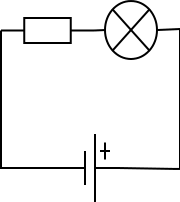
\includegraphics [width=.9\textwidth,keepaspectratio]{img/resistor_led.png}
			\end{center}
		\end{column}
		\begin{column}[c]{.5\textwidth}
\begin{Verbatim}[fontsize=\scriptsize]
#define LED_PIN 13

void setup () {
  pinMode (LED_PIN, OUTPUT);
}

void loop () {
  digitalWrite (LED_PIN, HIGH);
  delay (1000);
  digitalWrite (LED_PIN, LOW);
  delay (1000);
}
\end{Verbatim}
		\end{column}
	\end{columns}
\end{frame}

\begin{frame}[containsverbatim]{Code sample : resistor and photoresistor}
	\begin{columns}[c,onlytextwidth]
		\begin{column}[c]{.5\textwidth}
			\begin{center}
				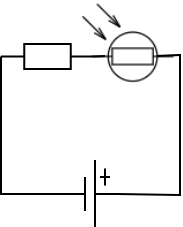
\includegraphics [width=.9\textwidth,keepaspectratio]{img/resistor_photoresistor.png}
			\end{center}
		\end{column}
		\begin{column}[c]{.5\textwidth}
\begin{Verbatim}[fontsize=\scriptsize]
#define LIGHT_SENSOR_PIN A0

void setup () {
  pinMode (LIGHT_SENSOR_PIN, INPUT);
  Serial.begin(9600);
}

void loop () {
  long sensorValue = 
    analogRead(LIGHT_SENSOR_PIN);

  Serial.print("Light Sensor : ");
  Serial.println(sensorValue);
  delay (1000);
}
\end{Verbatim}
		\end{column}
	\end{columns}
\end{frame}


\begin{frame}[containsverbatim]{Code sample : UDP with EthernetShield }
	\begin{columns}[c]
		\begin{column}[c]{.4\textwidth}

\begin{Verbatim}[fontsize=\scriptsize]
byte mac[] = {
  0xDE, 0xAD, 0xBE, 
  0xEF, 0xFE, 0xED };
IPAddress ip(192, 168, 1, 177);
void setup() {
  Ethernet.begin(mac,ip);
  Udp.begin(1234);
  Serial.begin(9600);
}
\end{Verbatim}

		\end{column}
		\begin{column}[c]{.8\textwidth}

\begin{Verbatim}[fontsize=\scriptsize]
void loop()
{
  int packetSize = Udp.parsePacket();
  if(packetSize)
  {
    Serial.print("Received packet of size ");
    Serial.println(packetSize);
  
    Udp.read(packetBuffer,UDP_TX_PACKET_MAX_SIZE);
    Serial.println("Contents:");
    Serial.println(packetBuffer);
  
    Udp.beginPacket(Udp.remoteIP(), Udp.remotePort());
    Udp.write(ReplyBuffer);
    Udp.endPacket();
  }
}
\end{Verbatim}

		\end{column}
	\end{columns}
\end{frame}

\begin{frame}{The IDE}
	\begin{center}
		\includegraphics<1> [width=1\textwidth,keepaspectratio] {img/ide_examples.png}
		\includegraphics<2> [width=1\textwidth,keepaspectratio] {img/ide_webserver.png}
		\includegraphics<3> [width=1\textwidth,keepaspectratio] {img/ide_webserver_buttons.png}
		\includegraphics<4> [width=1\textwidth,keepaspectratio] {img/ide_serial.png}
	\end{center}
\end{frame}

\begin{frame}{Documentation}
	On the arduino.cc website
	\begin{itemize}
		\item Simple, Readable, Relevant 
		\item open access (and edit) wiki, 
		\item regular updates
	\end{itemize}
\end{frame}

\begin{frame}{Documentation}
	For all pages about a subject, there are
	\begin{itemize}
		\item hardware scheme
		\item code samples, with relevant comments, Creative Common license
	\end{itemize}
\end{frame}

\begin {frame} {Examples}
	\begin {center}
		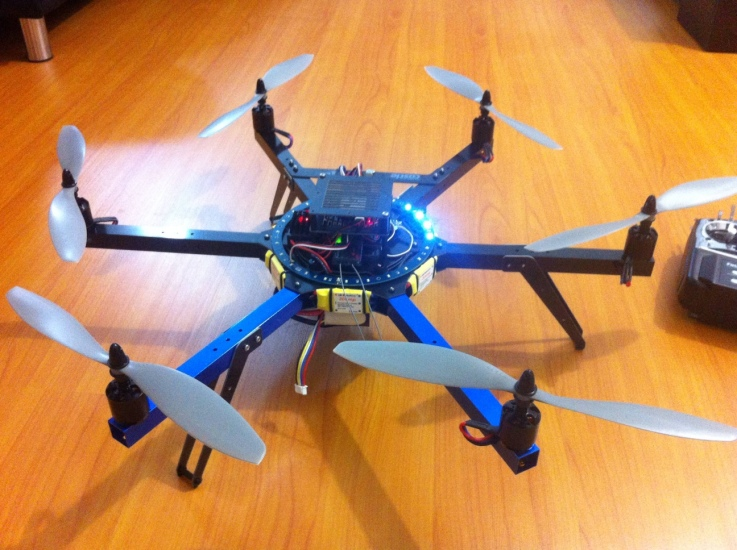
\includegraphics [width=.7\textwidth,keepaspectratio] {img/drone}
	\end {center}
\end {frame}

\begin {frame} {Examples}
	\begin {center}
		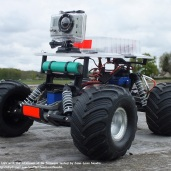
\includegraphics [width=.5\textwidth,keepaspectratio] {img/rover}
	\end {center}
\end {frame}
